\documentclass[12pt,a4paper]{report}
\usepackage{graphicx}
\usepackage{amsmath}
\usepackage{fancyhdr}
\usepackage{cite}
\usepackage{framed}
\usepackage{a4wide}
\usepackage{float}
\usepackage{epsfig}
\usepackage{longtable}
\usepackage{enumerate}
\usepackage{afterpage}
\usepackage{multirow}
\usepackage{ragged2e}
\usepackage{gensymb}
\usepackage{amsfonts} 
\usepackage[left=2 cm,top=2 cm,right=2 cm,bottom= 2cm]{geometry}
\usepackage{array}
\usepackage{setspace}           
\usepackage{float}
\usepackage{txfonts}
\usepackage{lipsum}
\usepackage{tikz}
\usetikzlibrary{calc}
\usepackage{subfiles} % Best loaded last in the preamble
\usepackage{adjustbox}
\newcommand{\Usefont}[1]{\fontfamily{#1}\selectfont}
\usepackage{lscape} % for landscape tables
\renewcommand{\baselinestretch}{1.7} 
\usepackage{array}
\usepackage{blindtext}
\usepackage{xpatch}
\usepackage{url}
\usepackage{leqno}
\usepackage{subcaption}
\usepackage{algorithm}
\usepackage{algpseudocode}

\linespread{1.5}
\usepackage[intoc, english]{nomencl}
\hyphenpenalty=5000
\tolerance=1000
\usepackage[nottoc]{tocbibind}
\bibliographystyle{IEEEtran}
\renewcommand{\bibname}{References}

%********************************************************
%*********************Figures*****************************
% Save all figures in the folder figures and include them in your 
% report using the command \includegraphics{figure-name}

\graphicspath{{figures/}}


\usepackage{lipsum}%% a garbage package you don't need except to create examples.
\usepackage{fancyhdr}
\pagestyle{fancy}
\lhead{}
\rhead{Computer Graphics Lab - Mini Project}
\cfoot{Department of Computer Science and Engineering}
\rfoot{\thepage}
\renewcommand{\headrulewidth}{2 pt}
\renewcommand{\footrulewidth}{2 pt}


\begin{document}
\gdef \title{VISVESVARAYA TECHNOLOGICAL UNIVERSITY
BELAGAVI-590018} % Seminar title
%*******************************************************************
% The font pages. The source tex files are there in the folder
%==================================coverpage.tex================================


\newenvironment{coverpage}
\thispagestyle{empty}
\begin{titlepage}
\subfile{design_cover}
   
		
	\begin{center}
		{\Usefont{phv} \Large \bf \title \par}
		\vspace*{10pt}
		 \centering
		\begin{figure}[h!]
			\centerline{
\includegraphics[scale=0.8]{vtu.png}}
		\end{figure}
		\large \em \Usefont{pzc}{ 
			A Database Management System Mini Project Report \\			on\\
			" Car Rental Management System "
			\\
			Submitted in partial fulfillment of the requirements for the V semester \\ 
			and award of the degree of \textbf{Bachelor of Engineering in Computer Science} \\and Engineering of Visvesvaraya Technological University, Belagavi }\\ [.15\baselineskip] \par
\begin{singlespace}
		Submitted by:\\
		\begin{center}
\begin{tabular}{ l l  }
 Aditya Sudhanshu  & 1RN20CS012\\ 
 Ayush Dixit  & 1RN20CS029\\
\end{tabular}
\end{center}
\centering
Under the Guidance of: \\
\bf{Prof. Karanam Sunil Kumar}
 \\ Assistant Professor \\ Dept. of CSE\\
		\begin{figure}[h!]
			\centerline{
\includegraphics[scale=0.8]{logo.png}}
		\end{figure}
		\vspace{\stretch{0.5}}
		\large{\bf Department of Computer Science and Engineering} \par
		\small{(NBA Accredited for academic years 2018-19, 2019-20, 2020-22)} \par
		\bf{RNS Institute of Technology}\\
\small{Channasandra, Dr.Vishnuvardhan Road, Bengaluru-560 098\\
2022-2023} \par
\end{singlespace}	
	\end{center}
\end{titlepage}	


 %Unless essential Do not edit this tex file



%%********************Certificate*******************

% To print name of only the seminar coordinator 1 in the certificate page
%==================================certificate1.tex================================
% To print name of only the seminar coordinator 1 in the certificate page

\newenvironment{certificate1}

	\clearpage\thispagestyle{empty}
	\subfile{design_cover}
	\begin{center}	
		%\vspace{1.5cm}
			\textbf{RNS Institute of Technology}\\
{\footnotesize{Channasandra, Dr.Vishnuvardhan Road, Bengaluru-560098}}\\
\textbf{DEPARTMENT OF COMPUTER SCIENCE  ENGINEERING} \\
{\footnotesize{(NBA Accredited for academic years 2022-25)}}\\
\end{center}
	
	\begin{center}
		
\includegraphics[scale=0.8]{logo.png}	
	\end{center}
	\begin{center}
		\textbf{CERTIFICATE}
	\end{center}
	
Certified that the mini project work entitled \textbf{“Car Rental Management System <”}has been successfully carried out by  \textbf{Aditya Sudhanshu} bearing USN  \textbf{"1RN20CS012"} and \textbf{Ayush Dixit} bearing USN  \textbf{"1RN20CS029"}, bonafide students of  \textbf{"RNS Institute of Technology"} in partial fulfillment of the requirements for the 6th semester  of  \textbf{"Bachelor of Engineering in Computer Science and Engineering of Visvesvaraya Technological University"}, Belagavi, during academic year 2022-2023. It is certified that all corrections/suggestions indicated for Internal Assessment have been incorporated in the report deposited in the departmental library. The project report has been approved as it satisfies the CG laboratory requirements of 6th semester BE, CSE. 	
\\
	
\vspace{1 cm}
\begin{center}

\begin{table}[ht]
%\begin{adjustbox}{width=1\textwidth}
\centering
\begin{tabular}{p{5.5cm} p{5.5cm} p{5.5cm} }
Signature of the Guide & Signature of the HoD & Signature of the Principal \\
\textbf{Prof. Karanam Sunil Kumar} & \textbf{Dr. Kiran}  & \textbf{Dr. M K Venkatesha}\\
Assistant Professor & Professor & Principal \\ 
Dept. of CSE  & Dept. of CSE & \\ 
\end{tabular}
%\end{adjustbox}

\end{table} 

\end{center}

\vspace{0.5cm}
\begin{flushleft}
External Viva:\\
Name of the Examiners         \hspace{5cm}          Signature with Date  \\
1.  \\
2. \\ 
			
\end{flushleft}
\thispagestyle{empty}




 

% To print names of both the seminar coordinators in the certificate page
%\include{certificate2} %Please uncomment this and comment the previous line

%%***************************************************



\pagenumbering{roman} 

%%********************************Abstract***********************
%==================================acknowledgement.tex=============================
\chapter*{Acknowledgement}%
\addcontentsline{toc}{chapter}{Acknowledgement}%

%\newenvironment{acknowledgement}
Any achievement, be it scholastic or otherwise does not depend solely on the individual 
efforts but on the guidance, encouragement and cooperation of intellectuals, elders and 
friends. A number of personalities, in their own capacities have helped us in carrying out 
this project work. We would like to take this opportunity to thank them all.\\
We are grateful to Management and \textbf{Dr. M K Venkatesha}, Principal, RNSIT, Bangalore, for his 
support towards completing this mini project.\\
We would like to thank \textbf{Dr. Kiran P}, Professor \& Head, Department of Computer 
Science \& Engineering, RNSIT, Bangalore, for his valuable suggestions and expert advice.\\
We deeply express our sincere gratitude to our guide \textbf{Prof. Karanam Sunil Kumar }, Assistant 
Professor, Department of CSE, RNSIT, Bangalore, for her able guidance, regular source of 
encouragement and assistance throughout this project. \\
We would like to thank all the teaching and non-teaching staff of Department of 
Computer Science \& Engineering, RNSIT, Bengaluru-98 for their constant support and encouragement.

\thispagestyle{plain}
 
%============================= abstract.tex================================
\chapter*{Abstract}%
%\addcontentsline{toc}{chapter}{\numberline{}Abstract}%
\addcontentsline{toc}{chapter}{Abstract}%


A car rental service allows individuals to rent a vehicle for a short period of time, typically by the day or week. Customers can choose from a variety of vehicles, including economy cars, luxury vehicles. Rental services may be offered by traditional brick-and-mortar businesses, as well as online companies. Some car rental companies also offer additional services such as GPS rentals and insurance options. The purpose of a car rental service is to provide customers with a convenient and flexible transportation option for their travel needs.\\
The objective of this project is making an interactive user-friendly website which makes the registration of new cars, their modification, deletion in an effective, easy way. Every entity can be easily searched according to date of requirement. We have implemented the idea by making a web application that includes table visualization. Any staff using the website will be able to insert all the details, update and delete them when needed. The UI has been made very simple to provide ease of access for all types of users.\\
This project requires HTML, CSS in the frontend, Php for backend and database connectivity and MySQL for database management. We seek to expand the project by having a fully real-life model of the department in the college. 
\thispagestyle{plain}
%=======================================================================

 

\thispagestyle{empty}
\newpage
    
%%**********************Table of Contents***********************
\tableofcontents
\thispagestyle{empty}
\newpage
\listoffigures
\listoftables
\cleardoublepage
\setcounter{page}{1}
\pagenumbering{arabic}

%%********************Chapters**********
\chapter{Introduction to Database Management System}
\section{Introduction}
Databases and database technology have a major impact on the growing use of computers. It is fair to say that databases play a critical role in almost all areas where computers are used, including business, electronic commerce, engineering, medicine, genetics, law, education, and library science. The word database is so commonly used that we must begin by defining what a database is. Our initial definition is quite general. A database is a collection of related data. By data, we mean known facts that can be recorded and that have implicit meaning. For example, consider the names, telephone numbers, and addresses of the people you know. You may have recorded this data in an indexed address book or you may have stored it on a hard drive, using a personal computer and software such as Microsoft Access or Excel. This collection of related data with an implicit meaning is a database. The preceding definition of database is quite general; for example, we may consider the collection of words that make up this page of text to be related data and hence to constitute a database. However, the common use of the term database is usually more restricted. 
A database has the following implicit properties:

\begin{itemize}
\item{A database represents some aspect of the real world, sometimes called the miniworld or the universe of discourse (UoD). Changes to the miniworld are reflected in the database.}
\item{A database is a logically coherent collection of data with some inherent meaning. A random assortment of data cannot correctly be referred to as a database}
\item{A database is designed, built, and populated with data for a specific purpose. It has an intended group of users and some preconceived applications in which these users are interested}
\end{itemize}
A database management system (DBMS) is a collection of programs that enables users to create and maintain a database. The DBMS is a general-purpose software system that facilitates the processes of defining, constructing, manipulating, and sharing databases among various users and applications. Defining a database involves specifying the data types, structures, and constraints of the data to be stored in the database. The database definition or descriptive information is also stored by the DBMS in the form of a database catalog or dictionary; it is called meta-data. Constructing the database is the process of storing the data on some storage medium that is controlled by the DBMS. Manipulating a database includes functions such as querying the database to retrieve specific data, updating the database to reflect changes in the miniworld, and generating reports from the data. Sharing a database allows multiple users and programs to access the database simultaneously.

\thispagestyle{fancy}


\section{ History of DBMS}
The history of database management systems (DBMS) can be traced back to the 1960s, when IBM developed the Integrated Data Store (IDS) for the U.S. Air Force. This was one of the first database management systems to be developed and used in a production environment.

In the 1970s, the relational model for databases was introduced by Dr. E.F. Codd at IBM. He proposed a new way of organizing data using tables with rows and columns, and a structured query language (SQL) for data manipulation. This model became the basis for the development of relational database management systems (RDBMS), such as IBM's System R and later, Oracle.

In the 1980s, the popularity of RDBMSs grew as personal computers became more powerful and affordable. This led to the development of several new RDBMSs, such as SQL Server, MySQL, and PostgreSQL.

In the 1990s, the internet and the World Wide Web emerged as a major new platform for information management and communication. This led to the development of new types of DBMSs, such as document databases and key-value stores, which are better suited for storing and retrieving unstructured data.

In recent years, NoSQL databases have gained popularity for their ability to handle large amount of unstructured data and also for their scalability, performance and ease of handling distributed data.

Overall, the history of DBMSs has been one of constant evolution, driven by advances in technology, changes in the way data is used and stored, and the emergence of new platforms and use cases.

\section{Applications of DBMS}
Applications where we use Database Management Systems are: \\
\begin{itemize}
\item \textbf{Telecom:} There is a database to keeps track of the information regarding calls made, network usage, customer details etc. Without the database systems it is hard to
maintain that huge amount of data that keeps updating every millisecond.
\item \textbf{Industry:} Where it is a manufacturing unit, warehouse or distribution centre, each one needs a database to keep the records of ins and outs. For example distribution
centre should keep a track of the product units that supplied into the centre as well as
the products that got delivered out from the distribution centre on each day; this is
where DBMS comes into picture.
\item \textbf{Banking System: } For storing customer info, tracking day to day credit and debit
transactions, generating bank statements etc. All this work has been done with the help
of Database management systems.
\item \textbf{Education Sector: } Database systems are frequently used in schools and colleges to store and retrieve the data regarding student details, staff details, course details, exam
details, payroll data, attendance details, fees details etc. There is a hell lot amount of
inter-related data that needs to be stored and retrieved in an efficient manner.
\item \textbf{Online Shopping: }You must be aware of the online shopping websites such as
Amazon, Flip kart etc. These sites store the product information, your addresses and
preferences, credit details and provide you the relevant list of products based on your
query. All this involves a Database management system.
\end{itemize}

 
\chapter{Tools and Technologies Used}
\section{HTML}
Hypertext Markup Language (HTML) is the standard markup language for creating web pages and web applications. With Cascading Style Sheets (CSS) and JavaScript it forms a triad of cornerstone technologies for the World Wide Web. Web browsers receive HTML documents from a web server or from local storage and render them into multimedia web pages. HTML describes the structure of a web page semantically and originally included cues for the appearance of the document.
HTML elements are the building blocks of HTML pages. With HTML constructs, images and other objects, such as interactive forms, may be embedded into the rendered page. It provides a means to create structured documents by denoting structural semantics for text such as headings, paragraphs, lists, links, quotes and other items. HTML elements are delineated by tags, written using angle brackets. Tags such as <img /> and <input /> introduce content into the page directly. Others such as <p>...</p> surround and provide information about document text and may include other tags as sub-elements. Browsers do not display the HTML tags, but use them to interpret the content of the page.
HTML can embed programs written in a scripting language such as JavaScript which affect the behavior and content of web pages. Inclusion of CSS defines the look and layout of content. 
\section{Bootstrap-A CSS Framework}
Cascading Style Sheets (CSS) is a style sheet language used for describing the presentation of a document written in a markup language. Although most often used to set the visual style of web pages and user interfaces written in HTML and XHTML, the language can be applied to any XML document, including plain XML, SVG and XUL, and is applicable to rendering in speech, or on other media. Along with HTML and JavaScript, CSS is a cornerstone technology used by most websites to create visually engaging webpages, user interfaces for web applications, and user interfaces for many mobile applications.

CSS is designed primarily to enable the separation of presentation and content, including aspects such as the layout, colors, and fonts. This separation can improve content accessibility, provide more flexibility and control in the specification of presentation characteristics, enable multiple HTML pages to share formatting by specifying the relevant CSS in a separate .css file, and reduce complexity and repetition in the structural content.

Bootstrap is a free and open-source front-end web framework used for  designing websites and web applications. It contains HTML- and CSS-based design templates for typography, forms, buttons, navigation and other interface components, as well as optional JavaScript extensions. Unlike many web frameworks, it concerns itself with front-end development only.

Bootstrap is the second most-starred project on GitHub, with more than 111,600 stars and 51,500 forks.
\section{Javascript}
JavaScript, often abbreviated as JS, is a high-level, interpreted programming language. It is a language which is also characterized as dynamic, weakly typed, prototype-based and multi-paradigm.

Alongside HTML and CSS, JavaScript is one of the three core technologies of the World Wide Web. JavaScript enables interactive web pages and this is an essential part of web applications. The vast majority of websites use it, and all major web browsers have a dedicated JavaScript engine to execute it.

As a multi-paradigm language, JavaScript supports event-driven, functional, and imperative (including object-oriented and prototype-based) programming styles. It has an API for working with text, arrays, dates, regular expressions, and basic manipulation of the DOM, but the language itself does not include any I/O, such as networking, storage, or graphics facilities, relying for these upon the host environment in which it is embedded.
\section{PHP}
PHP (Hypertext Preprocessor) is a server-side scripting language that is commonly used to create dynamic web pages. It is open-source software, which means that it can be freely modified and distributed. PHP is often used in conjunction with a web server like Apache and a database management system like MySQL, to create dynamic web applications.

PHP code can be embedded within HTML code, making it easy to create interactive and dynamic web pages. Some of the features of PHP include:
Variables: PHP supports a wide range of data types, including integers, strings, and arrays.
Functions: PHP has a large number of built-in functions that can be used to perform a wide range of tasks, such as working with strings, arrays, and dates.
Control Structures: PHP supports all of the standard control structures, such as if/else statements and loops.
Error handling: PHP has built-in error handling capabilities, which can be used to handle errors and exceptions in a consistent and controlled manner.
Database connectivity: PHP has built-in support for connecting to a wide range of databases, such as MySQL, Oracle, and Microsoft SQL Server.
Security: PHP provides several built-in functions and extensions to help secure your code from common security threats such as SQL injection, cross-site scripting (XSS), and cross-site request forgery (CSRF).

\section{MySQL}
MySQL is a widely used, open-source relational database management system (RDBMS). It is designed to store and manage large amounts of data in an efficient and organized manner. MySQL is particularly popular for web-based applications, due to its speed, reliability, and ease of use.
Some of the features of MySQL include:
SQL support: MySQL uses the SQL (Structured Query Language) to interact with the database, allowing developers to easily create, read, update, and delete data.
Tables and relationships: MySQL allows you to create multiple tables, each with its own structure and data, and to define relationships between them.
Indexes: MySQL allows you to create indexes on specific columns in a table to improve query performance.
Stored procedures and triggers: MySQL allows you to create stored procedures and triggers to automate repetitive tasks and enforce data integrity.
Security: MySQL supports a variety of security features, such as user management, encryption, and access control, to help protect data from unauthorized access.

%%********************Chapter 3**********

\chapter{Resource Requirements}
\section{Hardware Requirements}
Typically, a database server will require a fast CPU, sufficient memory, and fast storage. The CPU should be multi-core and have a high clock speed to handle the processing power required for a database. A minimum of 16GB of RAM is recommended, but more is needed for larger databases or more concurrent users.

Storage is also important for a database, as it needs to be fast and reliable. A solid-state drive (SSD) is recommended for the best performance, as it has faster read and write speeds compared to traditional hard disk drives (HDD). Additionally, the storage should be large enough to accommodate the size of the database and the growth rate.

Additionally, a database server also requires a reliable network connection, as it will be communicating with other systems and clients. A fast and stable network connection is important for ensuring that the data is transmitted quickly and reliably.

Finally, for high availability and disaster recovery, a database server can be clustered with multiple servers working together to provide redundancy and failover capabilities. This can be done using hardware or software solutions.
\section{Software Requirements} 
The software requirements for a database management system (DBMS) include the operating system, the DBMS software itself, and any additional tools or utilities that may be needed.

The operating system for a database server should be a stable and reliable platform that is well-suited for running database software. Some popular choices include Windows Server, Linux, and Unix. It's important to choose an operating system that is supported by the DBMS software you plan to use.

The DBMS software itself is the core component of the database system. There are many different DBMS software options available, such as MySQL, SQL Server, Oracle, PostgreSQL, and MongoDB. It's important to choose a DBMS that is compatible with your operating system and that meets your specific needs.

Additional tools or utilities that may be needed include backup and recovery software, monitoring and performance tuning tools, and data migration tools. These tools can help you manage and maintain your database, and ensure that it is running at optimal performance.
\section{Functional Requirements}
\subsection{Major Entities}
\textbf{CARS}: This includes information about the cars available for rental, such as make, model, year, and current availability.\\
\textbf{CUSTOMERS}:This includes information about the people who are renting the cars, such as name, contact information, and driver's license information.\\
\textbf{RESERVATION}: This includes information about the reservations that have been made, including the dates and times of the rental, the vehicle that has been reserved, and the customer who made the reservation.\\
\textbf{RENTALS}: This includes information about the actual rentals that have taken place, including the dates and times of the rental, the vehicle that was rented, the customer who rented it, and any additional charges or fees that may have been incurred.\\
\textbf{BILLING AND PAYMENT}: This includes information about the charges for the rentals, any additional fees, and the methods of payment that are accepted.\\
\textbf{EMPLOYEE}: This includes information about the employees of the car rental company, such as their name, contact information, and role within the company.\\
\subsection{End User Requirements}
\begin{enumerate}
\item Main Goals:
	\begin{itemize}
	\item Our motto is to develop a software program allowing customers to easily search for and book available vehicles online or through a web application.
	\item Hereby, The system should show customers the real-time availability of vehicles, so they can quickly and easily make a reservation.
	\end{itemize}
\item Flexibility:
	\begin{itemize}
	\item The system should offer customers a variety of rental options, such as daily, weekly, or monthly rentals, and should also allow for different pickup and drop-off locations.
	\end{itemize}		
\item Ease of use:
	\begin{itemize}
	\item The system should have a user-friendly interface that is easy to navigate and understand, making it simple for customers to find the information they need.	\end{itemize}
\end{enumerate}
\chapter{Database Design}
\section{Entities, Attributes and Relationships}
The database, called data, will have eight tables, books, borrowed\_cars, cars, categories, engine\_types, system\_settings, transmission\_types and users. Each will hold information about either the cars and bookings. The two
tables will be linked through a foreign key. The  table has the following fields:\\
\begin{figure}[H]
\centering
\caption{Car Rental table}
\includegraphics[scale=.9]{./Blank Diagram}
\\[0.2in]
\label{fig:Car Rental}
\end{figure}


\section{Identify Major entities, attributes and relationships}
\begin{itemize}
\item Login page to give access to priviledged Admin.
\item Adding car details details by the Admin.
\item Changing the id and password of the staffs.
which stores the details of transaction.
\item Admin can check all details  and modify them.
\item Admin can delete the entities in the tables.
\item Easy  search facilities to get the reqiured information.
\end{itemize}
\section{ER Schema}
\begin{figure}[H]
\centering
\caption{Entity Relationship Diagram}
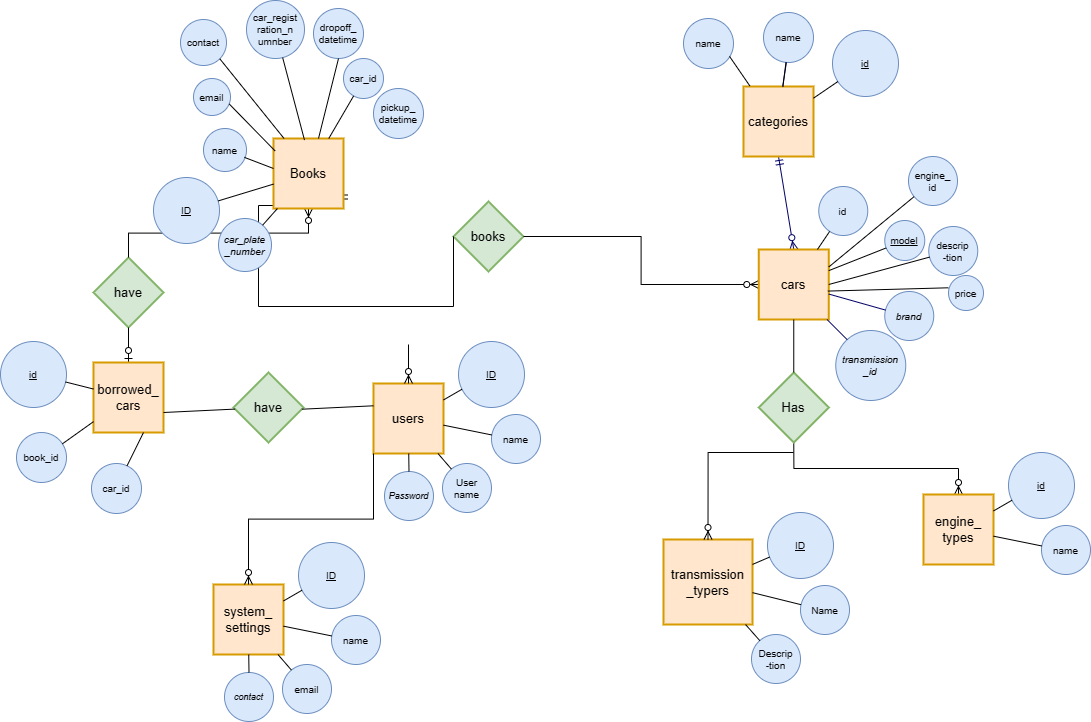
\includegraphics[width=\textwidth,height=\textheight,keepaspectratio]{./ER.png}
\\[0.2in]
\label{fig:Entitiy Relationship Diagram}
\end{figure}

\pagebreak
\thispagestyle{fancy}

\section{Schema Diagram}
\begin{figure}[H]
\centering
\caption{Relational Schema}
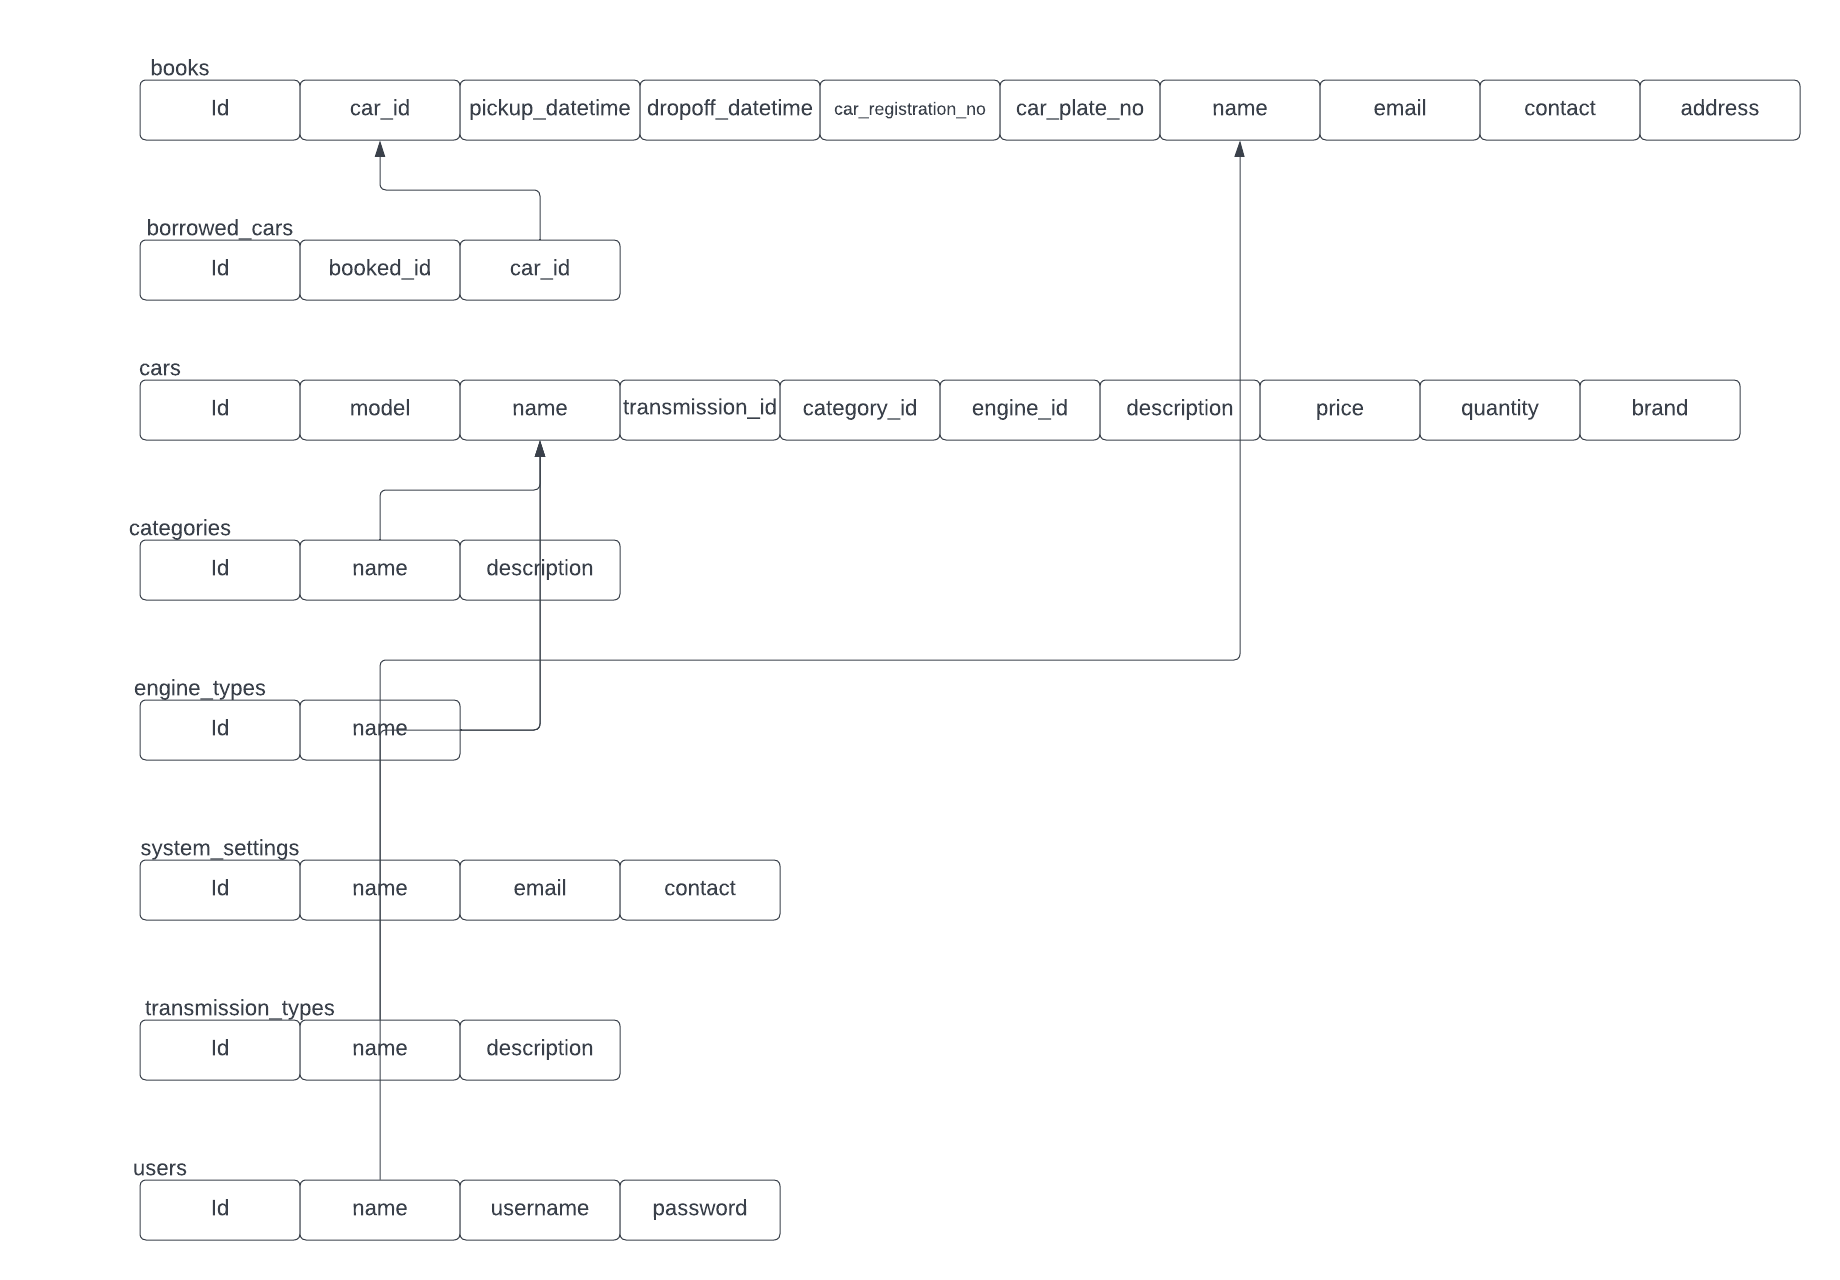
\includegraphics[scale=.65]{./Schema.png}
\\[0.2in]
\label{fig:Relational Schema}
\end{figure}

\thispagestyle{fancy}

\chapter{Implementation}
\section{PHP}
<!DOCTYPE html>
<html lang="en">
    <?php
    session\_start();
    include('admin/db_connect.php');
    ob_start();
        $query = $conn->query("SELECT * FROM system_settings limit 1")->fetch_array();
         foreach ($query as $key => $value) {
          if(!is_numeric($key))
            $_SESSION['system'][$key] = $value;
        }
    ob\_end\_flush();
    include('header.php');
    include('config.php');

	
    ?>

    <style>
    	header.masthead {
		  background: url(admin/assets/uploads/<?php echo $_SESSION['system']['cover_img'] ?>);
		  background-repeat: no-repeat;
		  background-size: cover;
		}
    
  #viewer_modal .btn-close {
    position: absolute;
    z-index: 999999;
    /*right: -4.5em;*/
    background: unset;
    color: white;
    border: unset;
    font-size: 27px;
    top: 0;
}
#viewer_modal .modal-dialog {
        width: 80%;
    max-width: unset;
    height: calc(90%);
    max-height: unset;
}
  #viewer_modal .modal-content {
       background: black;
    border: unset;
    height: calc(100%);
    display: flex;
    align-items: center;
    justify-content: center;
  }
  #viewer_modal img,#viewer_modal video{
    max-height: calc(100%);
    max-width: calc(100%);
  }
  body,main {
    background: #121212 !important;
    padding-bottom: 15px;
}
footer{
  background: #020202 !important;
}
 

a.jqte_tool_label.unselectable {
    height: auto !important;
    min-width: 4rem !important;
    padding:5px
}

#carousel-field{
    position: fixed;
    z-index: -1;
    width: calc(100%)
}
#carousel-field, #carsCarousel, #carsCarousel .carousel-inner,#carsCarousel .carousel-item,#carsCarousel img{
    /*max-height: 60vh*/
} 
.col-lg-8.align-self-end.mb-4.page-title {
    background: #00000070;
}

/*
a.jqte_tool_label.unselectable {
    height: 22px !important;
}*/
    </style>
    <?php 
        $page = isset($_GET['page']) ?$_GET['page'] : "home";
        if($page == 'home'):
     ?>
     <style>
       .masthead{
    background: unset!important
}
.masthead:before{
    content: unset!important;
}
     </style>
  <header class="masthead">
        <?php 
        $cars_img = scandir('admin/assets/uploads/cars_img/');
            foreach($cars_img as $k=> $fname){
                if(in_array($fname,array('.','..'))){
                    unset($cars_img[$k]);
                }
            }
            if(count($cars_img) > 0):
        ?>
        <div id="carousel-field">
        <div id="carsCarousel" class="carousel slide" data-ride="carousel">
          <div class="carousel-inner">
            <?php
            $i = 0 ;
             foreach($cars_img as $fname):
                $active = ($i == 0) ? 'active' : '';
                $i++;
            ?>
            <div class="carousel-item <?php echo $active ?>">
              <img class="d-block w-100" src="admin/assets/uploads/cars_img/<?php echo $fname ?>" alt="">
            </div>
            <?php endforeach; ?>
          </div>
        </div>
        </div>
    <?php endif; ?>

       <div class="container h-100">
            <div class="row h-100 align-items-center justify-content-center text-center">
                <div class="col-lg-8 align-self-end mb-4 page-title">
                  <h3 class="text-white">Welcome to Backchodi<?php echo $_SESSION['system']['name']; ?></h3>
                    <hr class="divider my-4" />

                <div class="col-md-12 mb-2 justify-content-center">
                  <form action="" id="find-car">
                    <div class="row form-group">
                      <div class="col-md-4">
                        <label for="" class="control-label text-white">Pickup Date/Time</label>
                        <input type="text" class="form-control datetimepicker" required="" name="pickup" autocomplete="off">
                      </div>
                      <div class="col-md-4">
                        <label for="" class="control-label text-white">Drop off Date/Time</label>
                        <input type="text" class="form-control datetimepicker" required="" name="dropoff" autocomplete="off">
                      </div>
                      <div class="col-md-4">
                        <label for="" class="control-label text-white">Category</label>
                        <select class="custom-select select2" name="category_id">
                          <option value="0">Any</option>
                          <?php
                          $qry = $conn->query("SELECT * FROM categories order by name asc");
                          while($row=$qry->fetch_assoc()):
                          ?>
                          <option value="<?php echo $row['id'] ?>"><?php echo $row['name'] ?></option>
                          <?php endwhile; ?>
                        </select>
                      </div>
                    </div>
                    <div class="form-group ">
                      <center>
                        <button class="btn btn-primary">Find Availability</button>
                      </center>
                    </div>
                  </form>
                </div>                        
                </div>
                
            </div>
        </div>  
    </header>
    <?php endif; ?>
    <body id="page-top">
        <!-- Navigation-->
        <div class="toast" id="alert_toast" role="alert" aria-live="assertive" aria-atomic="true">
        <div class="toast-body text-white">
        </div>
      </div>
        <nav class="navbar navbar-expand-lg navbar-light fixed-top py-3" id="mainNav">
            <div class="container">
                <a class="navbar-brand js-scroll-trigger" href="./"><?php echo $_SESSION['system']['name'] ?></a>
                <button class="navbar-toggler navbar-toggler-right" type="button" data-toggle="collapse" data-target="#navbarResponsive" aria-controls="navbarResponsive" aria-expanded="false" aria-label="Toggle navigation"><span class="navbar-toggler-icon"></span></button>
                <div class="collapse navbar-collapse" id="navbarResponsive">
                    <ul class="navbar-nav ml-auto my-2 my-lg-0">
                        <li class="nav-item"><a class="nav-link js-scroll-trigger" href="index.php?page=home">Home</a></li>
                        <li class="nav-item"><a class="nav-link js-scroll-trigger" href="index.php?page=about">About</a></li>
                       
                        
                     
                    </ul>
                </div>
            </div>
        </nav>
  <main>
        <?php 
        include $page.'.php';
        ?>
       
</main>
<div class="modal fade" id="confirm_modal" role='dialog'>
    <div class="modal-dialog modal-md" role="document">
      <div class="modal-content">
        <div class="modal-header">
        <h5 class="modal-title">Confirmation</h5>
      </div>
      <div class="modal-body">
        <div id="delete_content"></div>
      </div>
      <div class="modal-footer">
        <button type="button" class="btn btn-primary" id='confirm' onclick="">Continue</button>
        <button type="button" class="btn btn-secondary" data-dismiss="modal">Close</button>
      </div>
      </div>
    </div>
  </div>
  <div class="modal fade" id="uni_modal" role='dialog'>
    <div class="modal-dialog modal-md" role="document">
      <div class="modal-content">
        <div class="modal-header">
        <h5 class="modal-title"></h5>
      </div>
      <div class="modal-body">
      </div>
      <div class="modal-footer">
        <button type="button" class="btn btn-primary" id='submit' onclick="$('#uni_modal form').submit()">Save</button>
        <button type="button" class="btn btn-secondary" data-dismiss="modal">Cancel</button>
      </div>
      </div>
    </div>
  </div>
  <div class="modal fade" id="uni_modal_right" role='dialog'>
    <div class="modal-dialog modal-full-height  modal-md" role="document">
      <div class="modal-content">
        <div class="modal-header">
        <h5 class="modal-title"></h5>
        <button type="button" class="close" data-dismiss="modal" aria-label="Close">
          <span class="fa fa-arrow-righ t"></span>
        </button>
      </div>
      <div class="modal-body">
      </div>
      </div>
    </div>
  </div>
  <div class="modal fade" id="viewer_modal" role='dialog'>
    <div class="modal-dialog modal-md" role="document">
      <div class="modal-content">
              <button type="button" class="btn-close" data-dismiss="modal"><span class="fa fa-times"></span></button>
              <img src="" alt="">
      </div>
    </div>
  </div>
  <div id="preloader"></div>
        <footer class=" py-5">
            <div class="container">
                <div class="row justify-content-center">
                    <div class="col-lg-8 text-center">
                        <h2 class="mt-0 text-white">Contact us</h2>
                        <hr class="divider my-4" />
                    </div>
                </div>
                <div class="row">
                    <div class="col-lg-4 ml-auto text-center mb-5 mb-lg-0">
                        <i class="fas fa-phone fa-3x mb-3 text-muted"></i>
                        <div class="text-white"><?php echo $_SESSION['system']['contact'] ?></div>
                    </div>
                    <div class="col-lg-4 mr-auto text-center">
                        <i class="fas fa-envelope fa-3x mb-3 text-muted"></i>
                        <!-- Make sure to change the email address in BOTH the anchor text and the link target below!-->
                        <a class="d-block" href="mailto:<?php echo $_SESSION['system']['email'] ?>"><?php echo $_SESSION['system']['email'] ?></a>
                    </div>
                </div>
            </div>
            <br>
            <div class="container"><div class="small text-center text-muted"> © 2022 - MADE BY | <a href="https://github.com/ayushD123" target="_blank">AYUSH DIXIT</a></div></div>
        </footer>
        
       <?php include('footer.php') ?>
    </body>
    <script type="text/javascript">
      $('#login').click(function(){
        uni_modal("Login",'login.php')
      })
      $('.datetimepicker').datetimepicker({
          format:'Y-m-d H:i',
      })
      $('#find-car').submit(function(e){
        e.preventDefault()
        location.href = 'index.php?page=search&'+$(this).serialize()
      })
    </script>
    <?php $conn->close() ?>

</html>

\section{Backbone - HTML, Bootstrap, Javascript,}
\begin{lstlisting}[language=HTML]
<!DOCTYPE html>
<html lang="en">
  <head>
    <meta charset="utf-8">
    <meta name="viewport" content="width=device-width, initial-scale=1">
    <title>Student Information System</title>
    <!-- Bootstrap Core CSS -->
    <link href="{{ url_for('static', filename='vendor/bootstrap/css/bootstrap.min.css') }}" rel="stylesheet">
    <!-- MetisMenu CSS -->
    <link href="{{ url_for('static', filename='vendor/metisMenu/metisMenu.min.css') }}" rel="stylesheet">
    <!-- Custom CSS (INCLUDES DATATABLES)-->
    <link href="{{ url_for('static', filename='dist/css/sb-admin-2.css') }}" rel="stylesheet">
    <!-- Morris Charts CSS -->
    <link href="{{ url_for('static', filename='vendor/morrisjs/morris.css') }}" rel="stylesheet">
    <!-- Custom Fonts -->
    <link rel="stylesheet" href="https://stackpath.bootstrapcdn.com/font-awesome/4.7.0/css/font-awesome.min.css">
  </head>
  <body>
    <div id="wrapper">
      <!-- Navigation -->
      <nav class="navbar navbar-default navbar-static-top" role="navigation" style="margin-bottom: 0">
        <div class="navbar-header">
          <button type="button" class="navbar-toggle" data-toggle="collapse" data-target=".navbar-collapse">
          <span class="sr-only">Toggle navigation</span>
          <span class="icon-bar"></span>
          <span class="icon-bar"></span>
          <span class="icon-bar"></span>
          </button>
          <a class="navbar-brand" href="/">Student Information System</a>
        </div>
        <!-- /.navbar-header -->
        <ul class="nav navbar-top-links navbar-right">
          
          <li class="dropdown">
            <a class="dropdown-toggle" data-toggle="dropdown" href="#">
              <i class="fa fa-user fa-fw"></i> <i class="fa fa-caret-down"></i>
            </a>
            <ul class="dropdown-menu dropdown-user">
              <li><a href="/view"><i class="fa fa-user fa-fw"></i> {{ id }}</a>
            </li>
            <li class="divider"></li>
            <li><a href="/logout"><i class="fa fa-sign-out fa-fw"></i> Logout</a>
          </li>
        </ul>
        <!-- /.dropdown-user -->
      </li>
      <!-- /.dropdown -->
    </ul>
    <!-- /.navbar-top-links -->
    <div class="navbar-default sidebar" role="navigation">
      <div class="sidebar-nav navbar-collapse">
        <ul class="nav" id="side-menu">
          <li class="sidebar-search">
            <div class="input-group custom-search-form">
              <input type="text" class="form-control" placeholder="Search...">
              <span class="input-group-btn">
                <button class="btn btn-default" type="button">
                <i class="fa fa-search"></i>
                </button>
              </span>
            </div>
            <!-- /input-group -->
          </li>
          <li>
            <a href="/"><i class="fa fa-dashboard fa-fw"></i> Dashboard</a>
          </li>
          <li>
            <a href="/teachers"><i class="fa fa-user fa-fw"></i> Teachers</a>
          </li>
          <li>
            <a href="#"><i class="fa fa-institution fa-fw"></i> Students<span class="fa arrow"></span></a>
            <ul class="nav nav-second-level">
              <li>
                <li>
                  <a href="/students">Student List</a>
                </li>
                <li>
                  <a href="/attendance">Attendance</a>
                </li>
                <li>
                  <a href="/marksheet">Marksheet</a>
                </li>
              </li>
            </ul>
          </li>
          <li>
            <a href="/courses"><i class="fa fa-cloud fa-fw"></i> Courses</a>
          </li>
          <li>
            <a href="/branch"><i class="fa fa-flask fa-fw"></i> Branch</a>
          </li>
          <li>
            <a href="/semester"><i class="fa fa-hdd-o fa-fw"></i> Semester Details</a>
          </li>
          <!-- /.sidebar-collapse -->
        </div>
        <!-- /.navbar-static-side -->
      </nav>
      <div id="page-wrapper">
        <div class="row">
          <div class="col-lg-12">
            <h1 class="page-header">
            
              Undefined
            
            </h1>
          </div>
          <!-- /.col-lg-12 -->
        </div>
        <!-- /.row -->
        
          <h1>No content provided.</h1>
        
        <!-- /#page-wrapper -->
      </div>
      <!-- /#wrapper -->
      <!-- jQuery -->
      <script src="{{ url_for('static', filename='vendor/jquery/jquery.min.js') }}"></script>
      <!-- Bootstrap Core JavaScript -->
      <script src="{{ url_for('static', filename='vendor/bootstrap/js/bootstrap.min.js') }}"></script>
      <!-- Metis Menu Plugin JavaScript -->
      <script src="{{ url_for('static', filename='vendor/metisMenu/metisMenu.min.js') }}"></script>
      <script src="{{ url_for('static', filename='dist/js/sb-admin-2.js') }}"></script>
      <!-- DataTables JavaScript -->
      <script src="{{ url_for('static', filename='vendor/datatables/js/jquery.dataTables.min.js') }}"></script>
      <script src="{{ url_for('static', filename='vendor/datatables-plugins/dataTables.bootstrap.min.js') }}"></script>
      <script src="{{ url_for('static', filename='vendor/datatables-responsive/dataTables.responsive.js') }}"></script>
      <script>
      $(document).ready(function() {
      $('#dataTables').DataTable({
      responsive: true
      });
      });
      </script>
    </body>
  </html>
\end{lstlisting}
\pagebreak



%Paste your code(limited to 5 pages)\\
\chapter{Results \& Snapshots}
Add Project Snapshots with description
\begin{figure}[H]
\centering
\caption{Admin Log In}
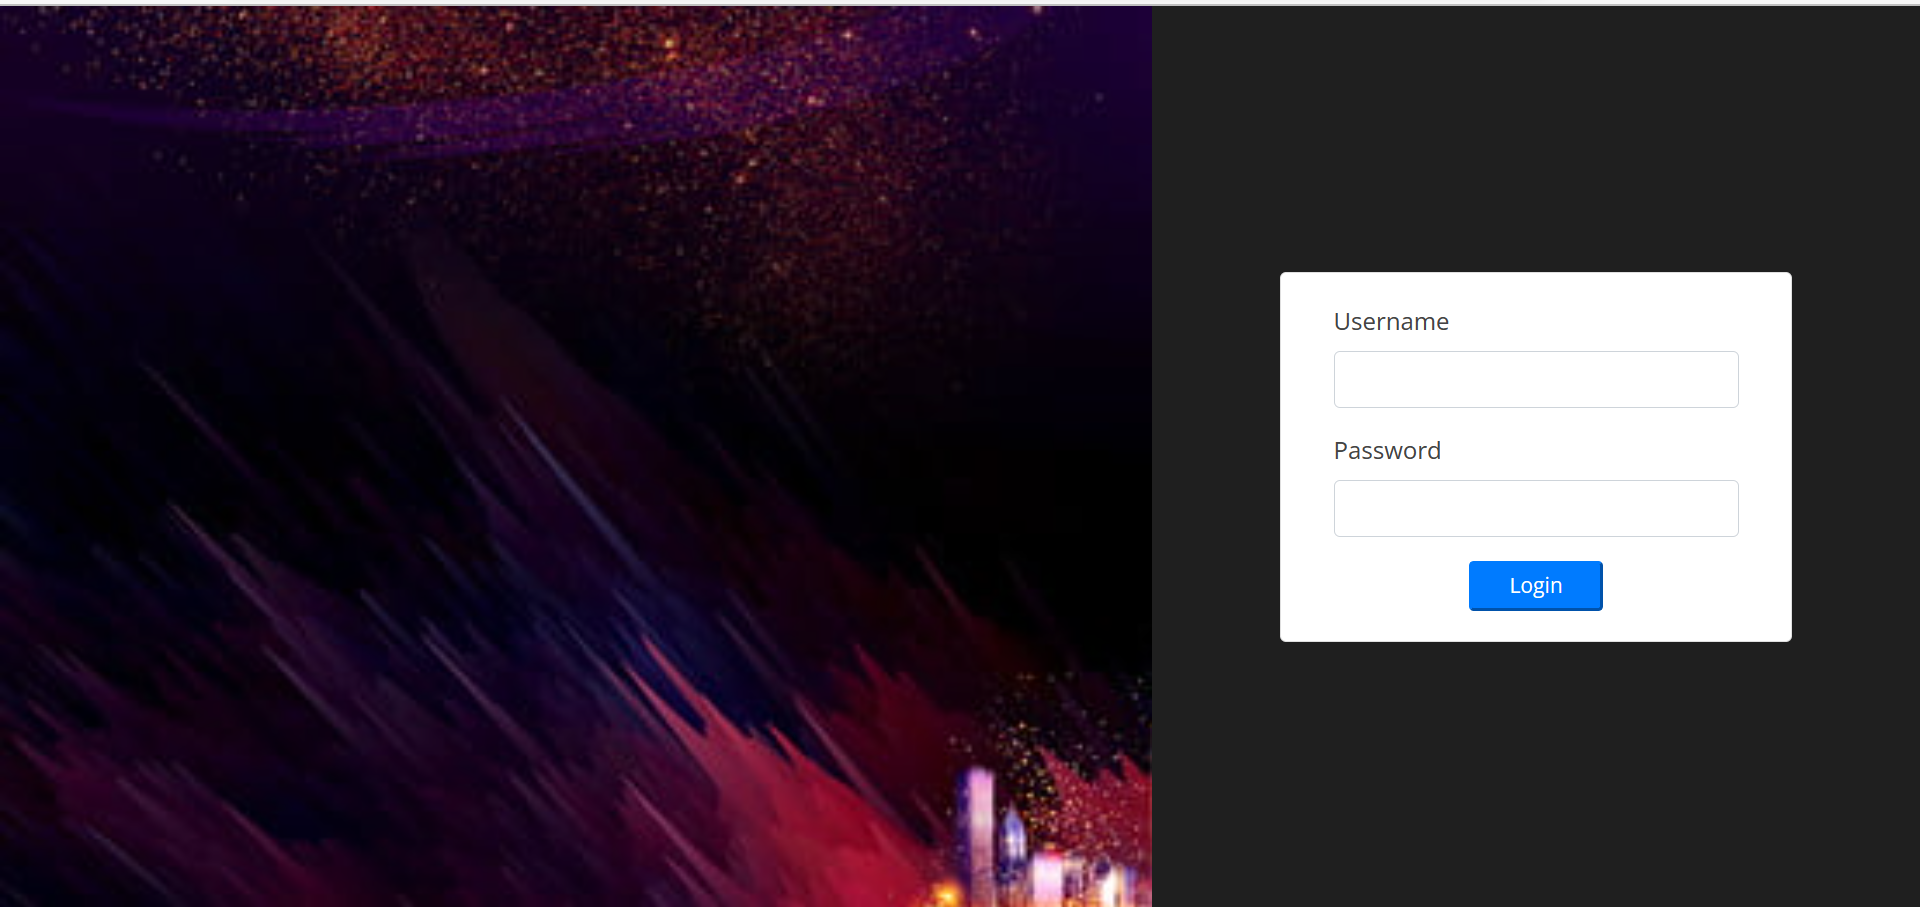
\includegraphics[width=\textwidth,height=\textheight,keepaspectratio]{admin-login.png}
\\[0.2in]
\label{fig:Login Form}
\end{figure}

\begin{figure}[H]
\centering
\caption{Landing Page}
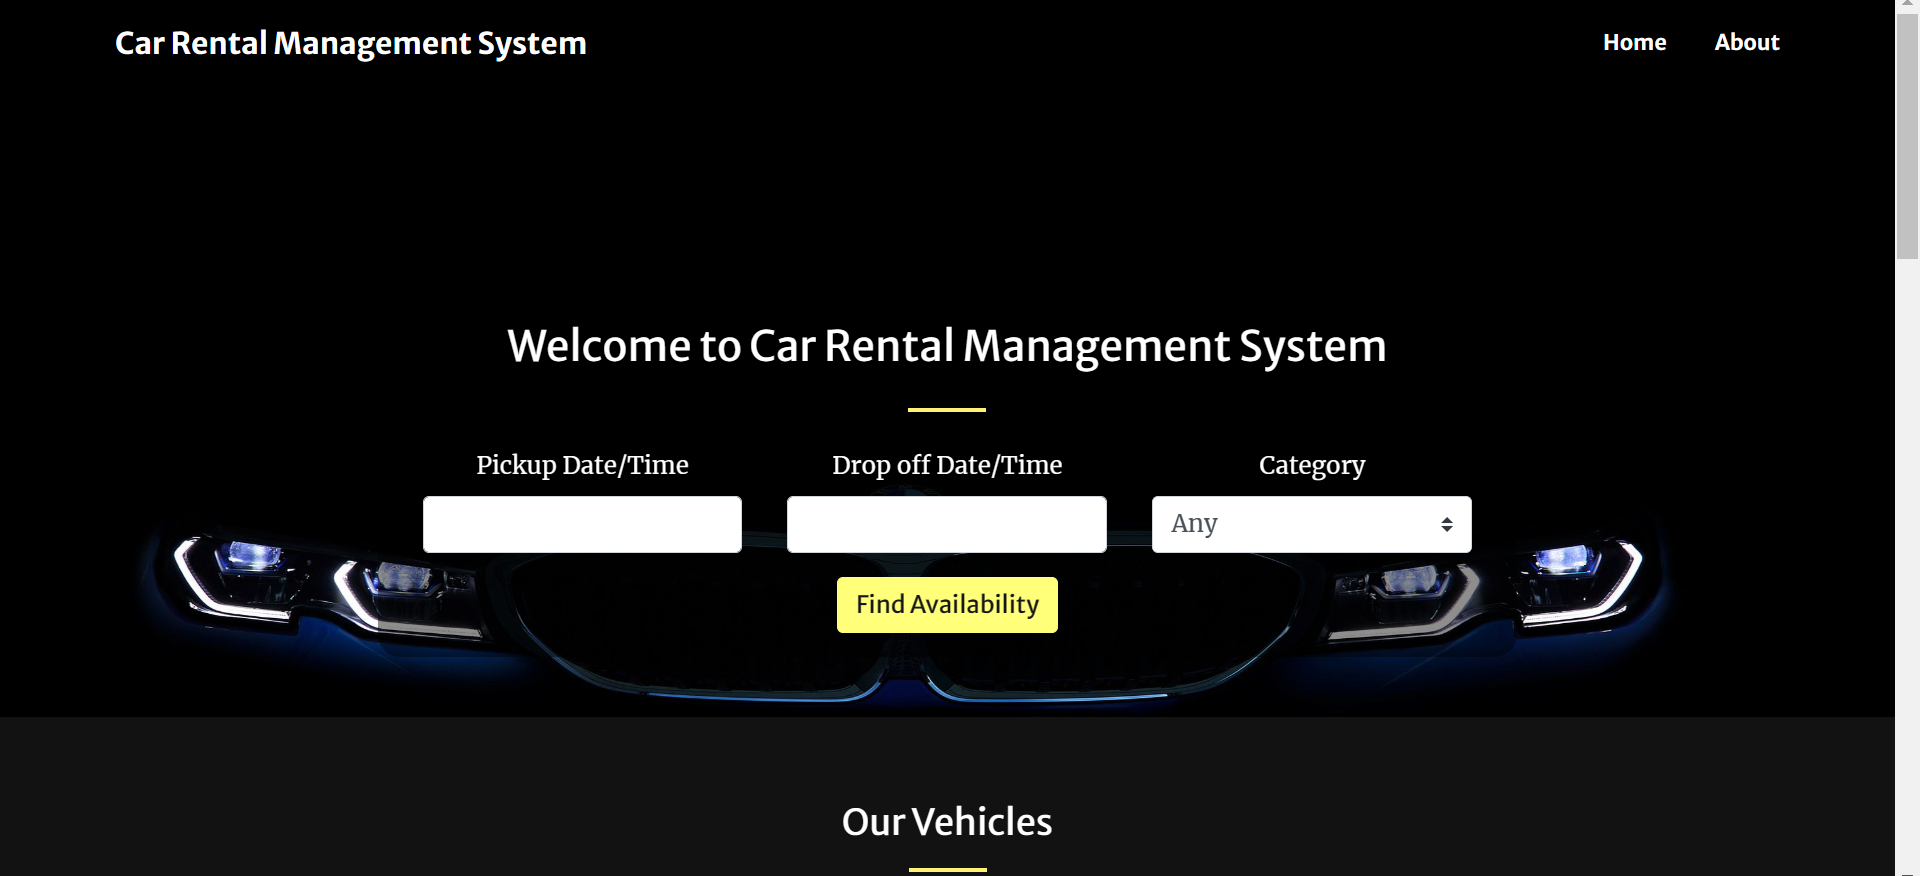
\includegraphics[width=\textwidth,height=\textheight,keepaspectratio]{landing page.png}
\\[0.2in]
\label{fig:Index Page}
\end{figure}
\begin{figure}[H]
\centering
\caption{Admin Dashboard}
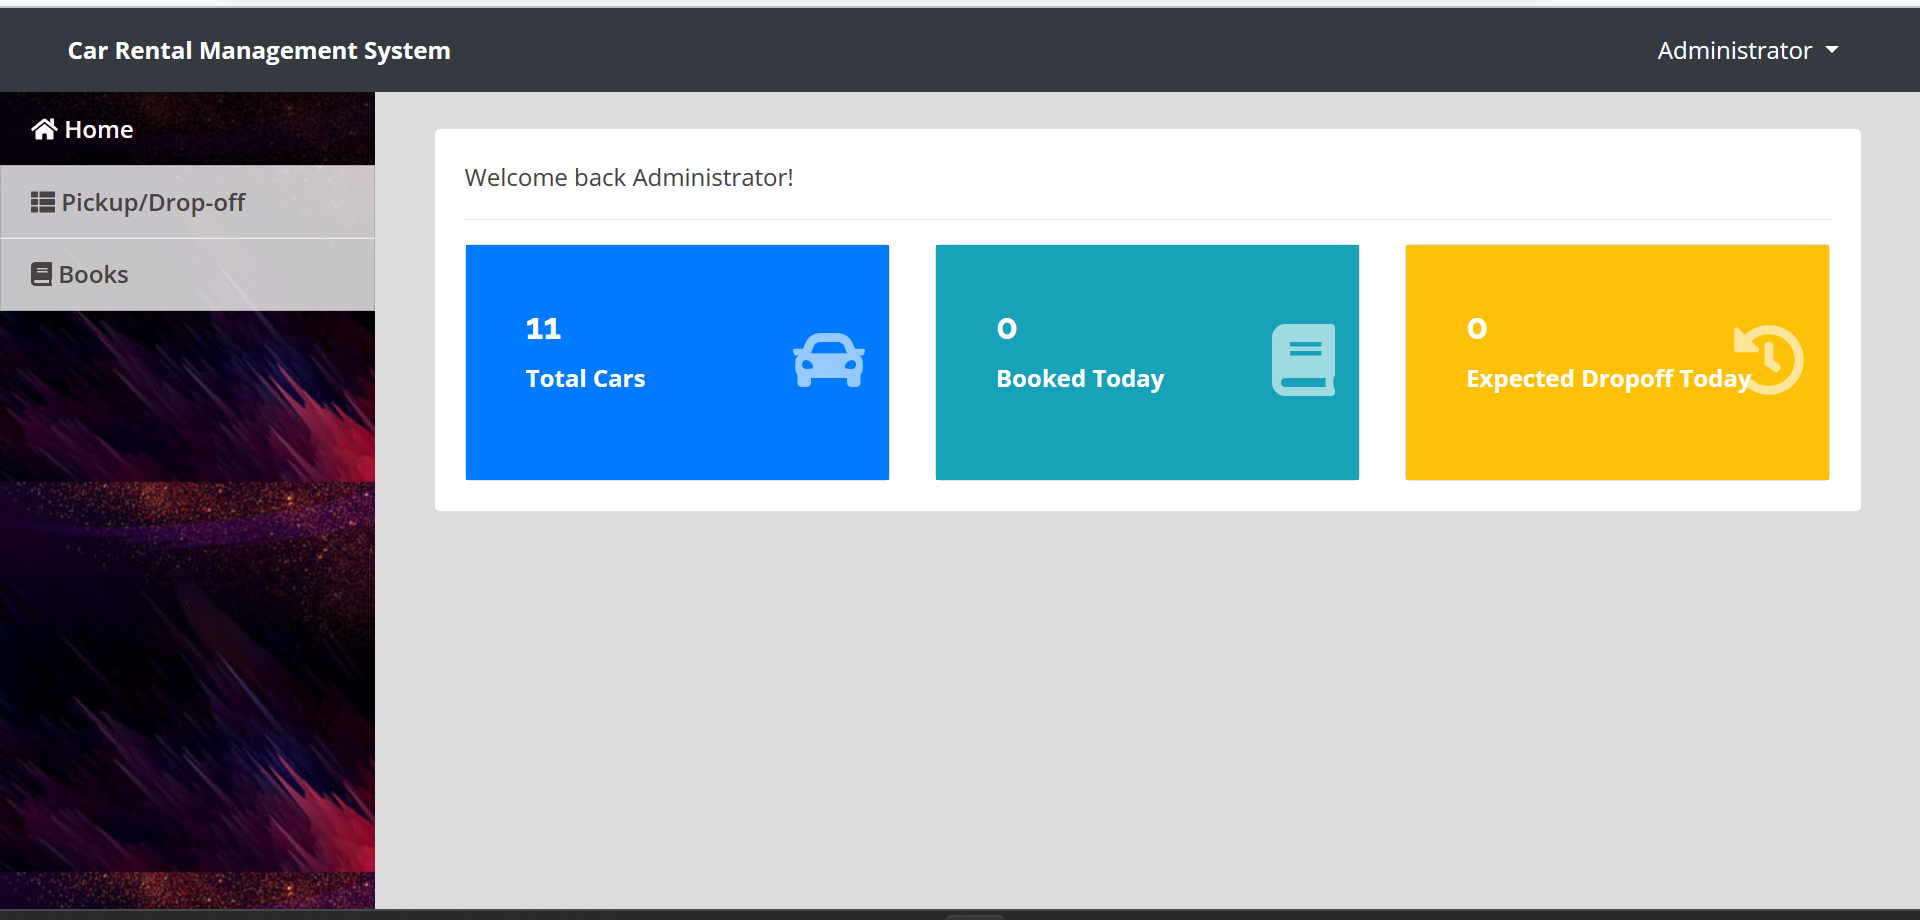
\includegraphics[width=\textwidth,height=\textheight,keepaspectratio]{admin dashboard.png}
\\[0.2in]
\label{fig:Teacher Details}
\end{figure}

\begin{figure}[H]
\centering
\caption{Pickup/dropoff}
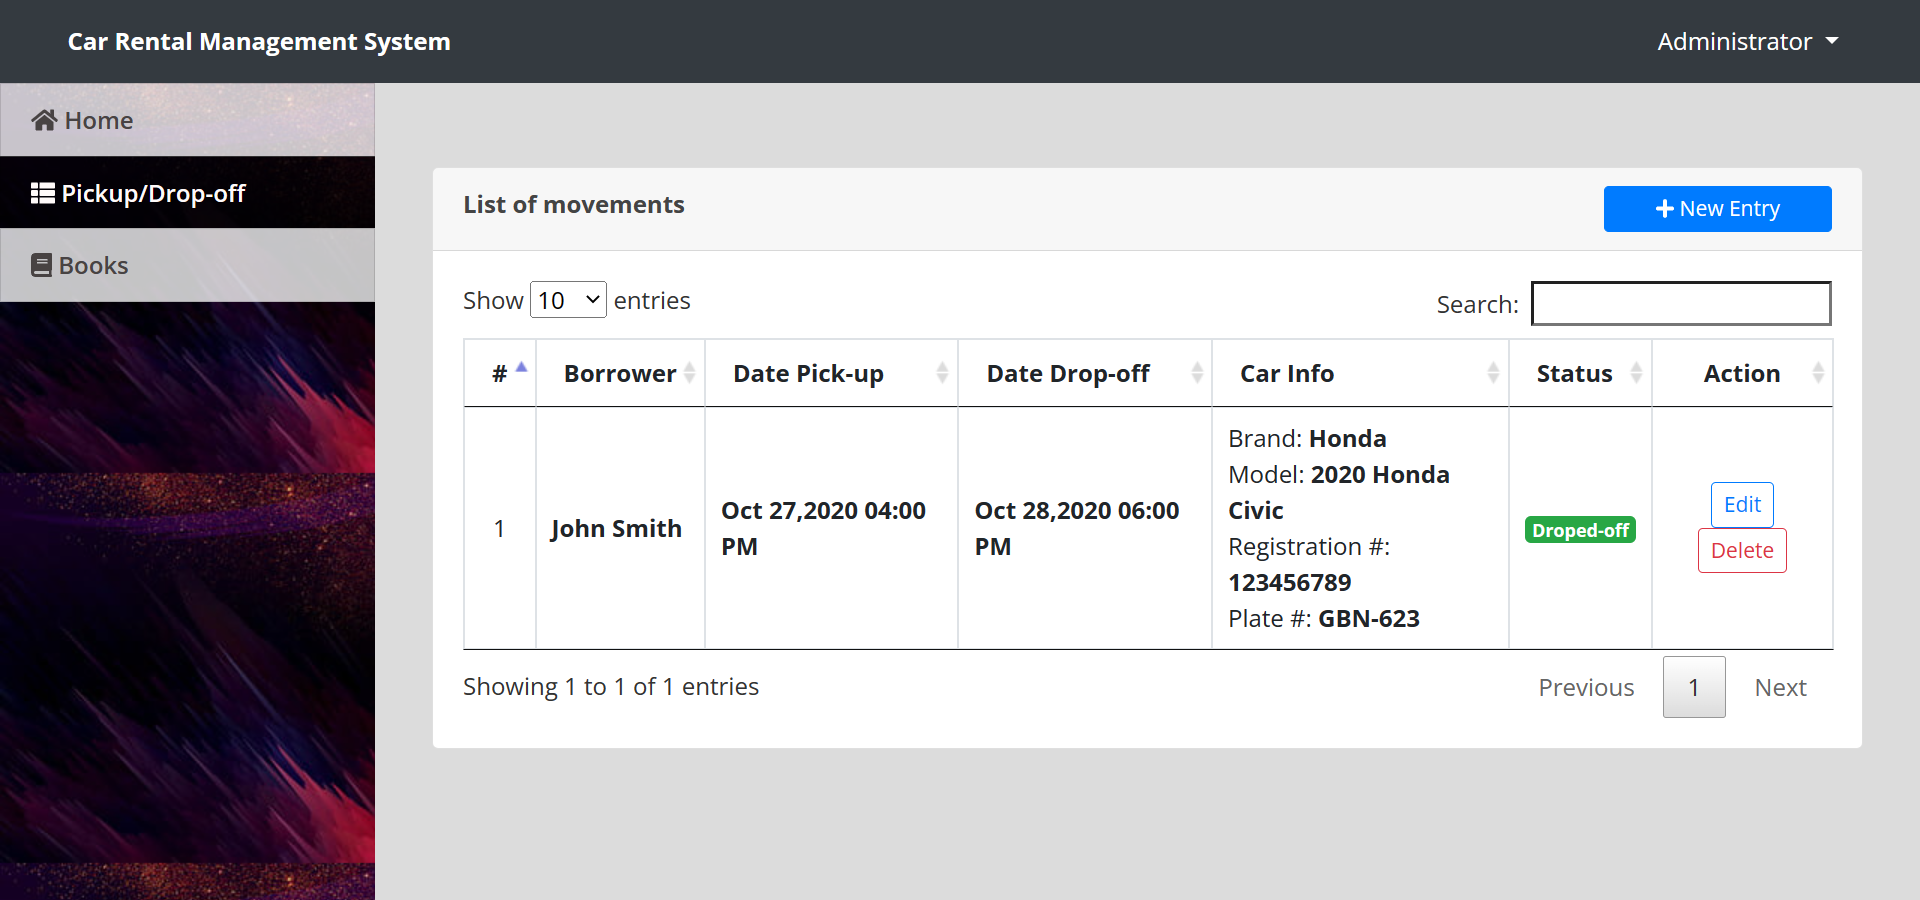
\includegraphics[width=\textwidth,height=\textheight,keepaspectratio]{pickupdropoff-table.png}
\\[0.2in]
\label{fig:Add Teacher}
\end{figure}
\begin{figure}[H]
\centering
\caption{Cars}
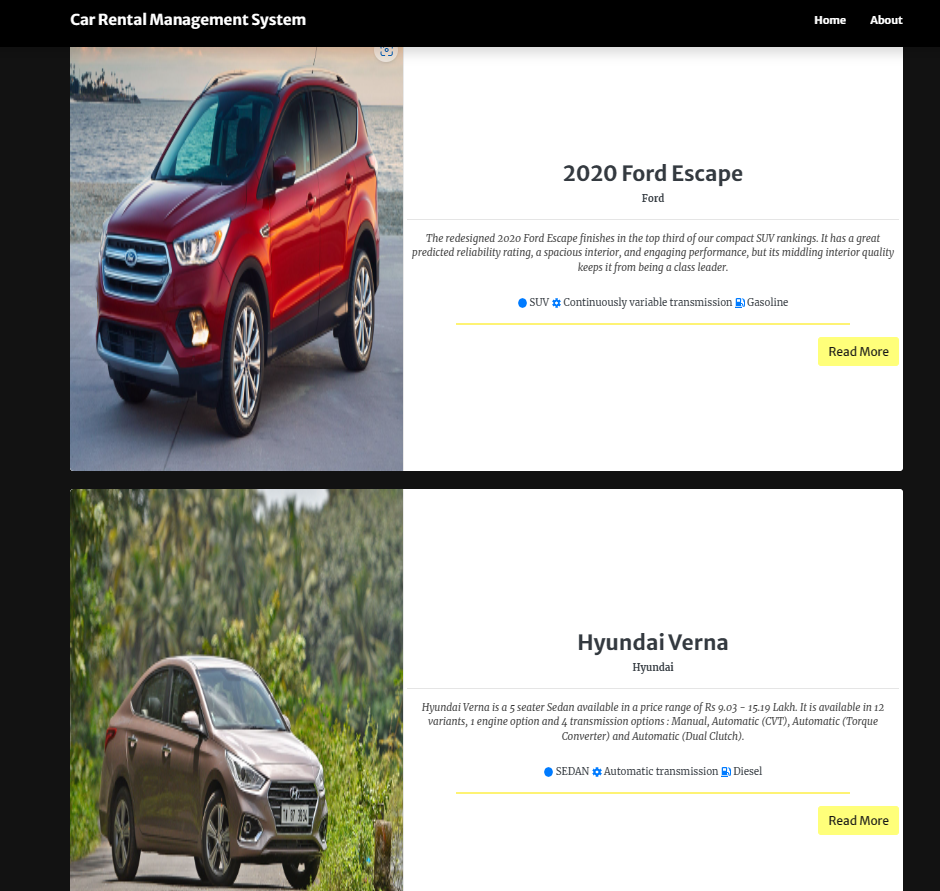
\includegraphics[width=0.65\textwidth,height=\textheight,keepaspectratio]{cars.png}
\\[0.1in]
\label{fig:Student Details}
\end{figure}
\begin{figure}[H]
\centering
\caption{Booking}
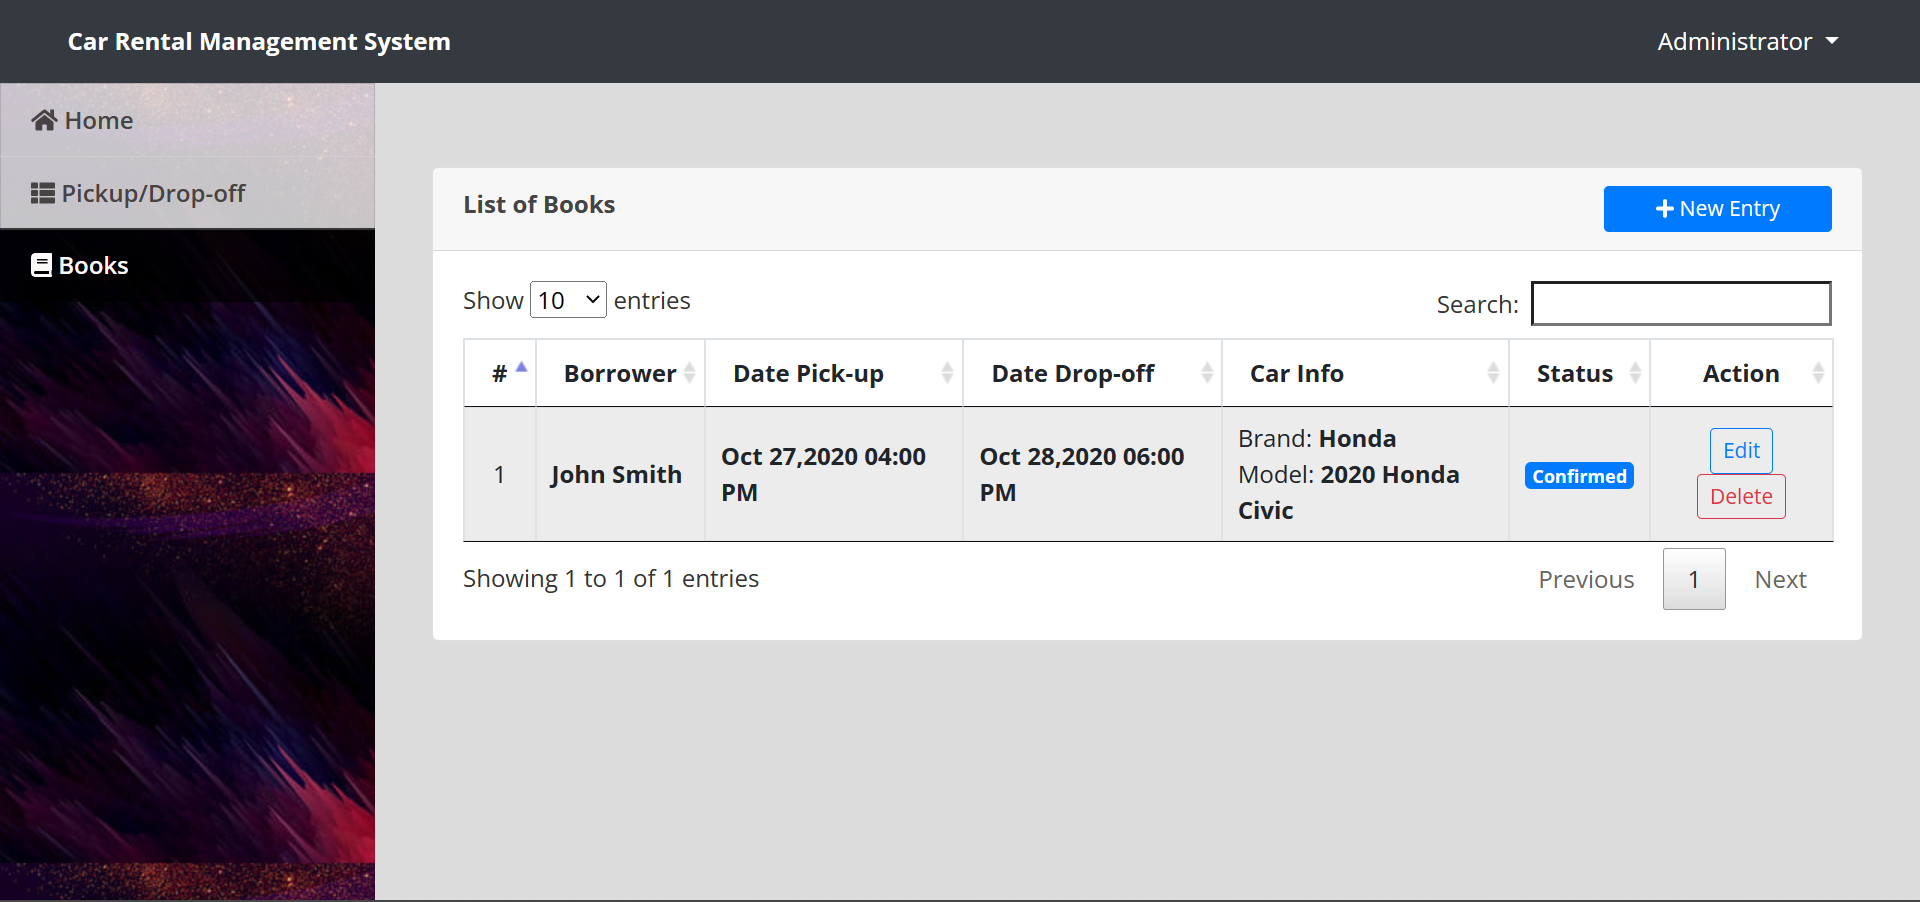
\includegraphics[width=\textwidth,height=\textheight,keepaspectratio]{booking-table.png}
\\[0.2in]
\label{fig:Attendance}
\end{figure}



\include{Chapter7}
%%********************Chapter 4**********
\chapter{Conclusion \& Future Enhancements}
\section{Conclusion}
A car rental management system is a software application that is designed to manage the operations of a car rental business. It typically includes features such as vehicle management, customer management, reservation management, billing and payment, and reporting.

The key entities in a car rental management system include vehicles, customers, reservations, rentals, billing and payment, and employees. These entities are typically stored in a relational database, such as MySQL, and accessed through a server-side scripting language, such as PHP.

The end user requirements for a car rental management system include easy and convenient booking, real-time availability, flexible rental options, multiple payment options, a user-friendly interface, security, and reporting.

The front-end of a car rental management system is typically created using a combination of HTML, CSS, and JavaScript, with the help of frameworks such as React, Angular, or Vue.js. The front-end communicates with the back-end to retrieve data from the database and display it to the user.

In conclusion, a car rental management system is a powerful tool that can automate and streamline the operations of a car rental business, making it more efficient and profitable. It is important to choose a system that meets the specific needs of your business and to implement it using best practices for security, performance, and scalability.
\pagebreak
\section{Future Enhancements}
There are several areas where car rental management services can be enhanced in the future:


1.Self-Service Kiosks: Self-service kiosks can be installed at the rental locations, allowing customers to quickly and easily rent cars without the need for human interaction.

2.Mobile App Integration: Car rental companies can develop mobile apps that allow customers to book cars, track their rental status, and make payments using their smartphones.

3.Automated Vehicle Management: Automated systems can be implemented to track the location, condition, and availability of rental cars in real-time, making it easier to manage the fleet and ensure that cars are always available for customers.

4.Predictive Maintenance: Predictive maintenance systems can be used to predict when a car will need maintenance and schedule it in advance, reducing downtime and keeping the fleet in top condition.

5.Advanced Payment Systems: Car rental companies can implement advanced payment systems that allow customers to make payments using various methods such as credit card, debit card, mobile wallet, and digital currencies.

6.Automated Return: Automated systems can be implemented to manage the return process of the cars, allowing customers to drop off their cars without having to interact with staff.

7.Virtual Reality: Virtual Reality can be used to give customers a virtual tour of the cars before renting them


%%********************References**********
%%****This template uses IEEE bibliography style
\begin{thebibliography}{99}

\bibitem{}Fundamentals of database systems by (Elmasri Navathe, 2000)\\
Article: Student Information System: \url{https://en.wikipedia.org/wiki/Student_information_system}

\bibitem{} Learning SQLite : \url{https://www.tutorialspoint.com/sqlite/}\\
Python and Flask tutorials : \url{http://flask.pocoo.org/docs/0.12/}, \url{http://www.youtube.com}

\bibitem{} Python : \url{https://docs.python.org/3/}

\bibitem{} ER Diagram and Schema : \url{https://erdplus.com}

\bibitem{} Stack Overflow: \url{https://stackoverflow.com/}

\end{thebibliography}

\end{document}